% \documentclass[12pt]{article}
\documentclass[12pt]{ctexart}
\usepackage[utf8]{inputenc}

\usepackage[english]{babel}
\usepackage[dvips]{epsfig}
\usepackage{amsmath}
\usepackage{amssymb}
\usepackage{amsfonts}
\usepackage{amsthm}
\usepackage{amsbsy}
\usepackage{amsgen}
\usepackage{amscd}
\usepackage{amsopn}
\usepackage{amstext}
\usepackage{amsxtra}
\usepackage{mathrsfs}
\usepackage{enumitem}
\usepackage{graphicx}
\usepackage{verbatim}
\usepackage{epstopdf}
\usepackage{float}
\usepackage[all,cmtip]{xy}
\usepackage{accents}
\usepackage{sseq}
\usepackage{url}
\usepackage{hyperref}
\usepackage{makeidx}
\usepackage{siunitx}
\usepackage{xcolor}
\usepackage{physics}

%%%%%%%%% 版面设置 %%%%%%%%%%%%%%%%%%%%%%%%%%%%%%%%%%%%%%
\usepackage{geometry}
\usepackage{titlesec}
\usepackage{fancyhdr}\pagestyle{empty}
\titleformat*{\section}{\large\bfseries}

%
\geometry{
	a4paper,
	total={170mm,240mm},
	left=20mm,
	top=30mm,
}

%Bitte nicht einstellen
\renewcommand{\figurename}{Abbildung}
\renewcommand{\tablename}{Tabelle}
\pagestyle{fancyplain}
\headheight 35pt
\lhead{\name}
\chead{\textbf{\Large \Title}}
\rhead{\due\\\today}
\lfoot{}
\cfoot{}
\rfoot{\small\thepage}
\headsep 1.5em

%%%%%%%%%%%%%%%%%%%%%%%%%%%%%%%%%%%%%%%%%%%%%%%%%%%%%%

\newtheorem{thm}{Theorem}[section]

% 定义解题环境
\theoremstyle{remark}
\newtheorem{remark}[thm]{Remark}
\newtheorem{theorem}{Theorem}
\newtheorem{observation}[thm]{Observation}

\theoremstyle{definition}
\newtheorem{problem}{\text{}}
\newtheorem{Problem}{\text{Problem}}
\newtheorem*{solution}{解}
\newtheorem*{Answer}{Answer}
\newtheorem{example}{Example} 

%%%%%%%%%%%%%%%%%%%%%%%%%%%%%%%%%%%%%%%%%%%%%%%%%%%%%%%%%%%%%%%%%%
\newcommand\name{陈景龙22120307}
\newcommand\due{-}
\newcommand{\emptyline}{\vspace{0.6\baselineskip}}

\usepackage{tikz}
\usepackage{array,tabularx}

\newcommand{\Title}{CVX HW}
\renewcommand{\due}{due: 11 weeks}
\newcommand{\dom}{\operatorname{dom}} % 定义域
\newcommand{\diag}{\operatorname{diag}} % 创建对角阵
\newcommand{\minimize}{\operatorname{minimize}} % 最小化
\newcommand{\maximize}{\operatorname{maximize}} % 最大化
\newcommand{\subject}{\operatorname{subject\ to}}

\newcommand{\todo}{{\color{red} to do}} % to do
\newcommand{\myline}{{\line(1,0){450}}} % 分割线

% 自定义 enumerate
\renewcommand{\labelenumi}{(\alph{enumi})}

\begin{document}
\section{Convex sets}
\begin{problem}[2.1]
    Let $C \subseteq \mathbb{R}^{n}$ be a convex set, with $x_1, \dots, x_k \in C$, and let $\theta_1, \dots, \theta_k \in \mathbb{R}$ satisfy $\theta_i \ge 0$, $\theta_1 + \cdots + \theta_k = 1$. Show that $\theta_1x_1 + \cdots + \theta_kx_k \in C$.(The definition of convexity is that this holds for $k = 2$; you must show it for arbitrary k.) \textit{Hint.} Use induction on k.

    \begin{proof}
        \text{}
        \begin{itemize}
            \item When $k = 2$, $\theta_i \ge 0, \theta_1 + \theta_2 = 1 \Longrightarrow \theta_1 x_1 + \theta_2x_2 = \theta_1 x_1 + (1 - \theta_1)x_2 \in C$.
            \item If $k = n$, $\theta_i \ge 0, \theta_1 + \cdots + \theta_n = 1 \Longrightarrow \theta_1x_1 + \cdots + \theta_nx_n \in C$ holds.
            \item Then $k = n + 1$, $\theta_i \ge 0, \theta_1 + \cdots + \theta_{n + 1} = 1 \Longrightarrow \theta_1x_1 + \cdots + \theta_nx_n + \theta_{n + 1}x_{n + 1} = (\theta_1 + \cdots + \theta_n)\frac{\theta_1x_1 + \cdots + \theta_nx_n}{\theta_1 + \cdots + \theta_n} + \theta_{n + 1}x_{n + 1}$. $k = n, \theta_1x_1 + \cdots + \theta_nx_n \in C$ holds, and $k = 2$ holds, so $\theta_1x_1 + \cdots + \theta_nx_n + \theta_{n + 1}x_{n + 1} \in C$.
            \item so $\theta_1x_1 + \cdots + \theta_kx_k \in C$ for arbitrary $k$.
        \end{itemize}
    \end{proof}
\end{problem}

\begin{problem}[2.5]
    What is the distance between two parallel hyperplanes $\left\{x \in \mathbb{R}^n | a^Tx = b_1\right\}$ and $\left\{x \in \mathbb{R}^n| \right.$ $\left. a^Tx = b_2\right\}$?

    \Answer The distance between the two hyperplanes is $\frac{|b_1 - b_2|}{\|a\|_2}$.
\end{problem}

\begin{problem}[2.11]
    \textit{Hyperbolic sets.} Show that the \textit{Hyperbolic set} $\left\{x \in \mathbb{R}_+^2 | x_1x_2 \ge 1\right\}$ is convex. As a generalization, show that $\left\{x \in \mathbb{R}^n_+ | \prod_{i = 1}^n x_i \ge 1\right\}$ is convex. \textit{Hint.} If $a, b \ge 0$ and $0 \le \theta \le 1$, then $a^\theta b^{1 - \theta} \le \theta a + (1 - \theta)b$.
    
    \Answer \begin{enumerate}
        \item $x, y \in C$, then $z = \theta x + (1 - \theta)y$.
        \begin{align*}
            z_1z_2 &= (\theta x_1 + (1 - \theta)y_1)(\theta x_2 + (1 - \theta)y_2) \\
            &\ge x_1^\theta y_1^{1 - \theta} \cdot x_2^\theta y_2^{1 - \theta} \\
            &= (x_1x_2)^\theta (y_1y_2)^{1 - \theta}\\
            &\ge 1
        \end{align*}
        we get $z \in C$ and $\left\{x \in \mathbb{R}_+^2 | x_1x_2 \ge 1\right\}$ is convex.
        \item $x, y \in C$, then $z = \theta x + (1 - \theta)y$.
        \begin{align*}
            z_1z_2 &= \prod_{i = 1}^n(\theta x_i + (1 - \theta)y_i)\\
            &\ge \prod_{i = 1}^n x_i^\theta y_i^{1 - \theta} \\
            &\ge 1
        \end{align*}
        we get $z \in C$ and $\left\{x \in \mathbb{R}^n_+ | \prod_{i = 1}^n x_i \ge 1\right\}$ is convex.
    \end{enumerate}
\end{problem}

\begin{problem}[2.14]
    \textit{Erpanded and restricted sets.} Let $S \subseteq \mathbb{R}^{n}$, and let $\|\cdot\|$ be a norm on $\mathbb{R}^n$.
    \begin{enumerate}
        \item For $a \ge 0$ we define $S_a$ as $\{x \mid \operatorname{dist}(x, S) \leq a\}$, where $\operatorname{dist}(x, S) = \inf_{y\in S}\|x - y\|$. We refer to $S_a$ as $S$ \textit{expanded} or \textit{extended} by $a$. Show that if $S$ is convex, then $S_a$ is convex.
        \item For $a \ge 0$ we define $S_{-a} = \left\{x | B(x, a) \subseteq S\right\}$, where $B(x, a)$ is the ball (in the norm $\|\cdot\|$), centered at x, with radius a. We refer to $S_{-a}$ as $S$ \textit{shrunk} or \textit{restricted} by $a$, since $S_{-a}$ consists of all points that are at least a distance a from $\mathbb{R}^n\backslash S$. Show that if $S$ is convex, then $S_{-a}$ is convex.
    \end{enumerate}

    \begin{proof}
        \begin{enumerate}
            \item $\forall x_1, x_2 \in S_a$, for $0 \le \theta \le 1$, $z = \theta x_1 + (1 - \theta)x_2$
            \begin{align*}
                \operatorname{dist}(z, S) &= \inf_{y\in S}\|z - y\|\\
                &= \inf_{y_1, y_2\in S}\|\theta x_1 + (1 - \theta)x_2 - \theta y_1 - (1 - \theta)y_2\|\\
                &\le \inf_{y_1, y_2\in S} (\theta\|x_1 - y_1\| + (1 - \theta)\|x_2 - y_2\|)\\
                &=\theta \inf_{y_1 \in S}\|x_1 - y_1\| + (1 - \theta) \inf_{y_2 \in S} \|x_2 - y_2\|\\
                &\le a
            \end{align*}
            so $\forall x_1, x_2 \in S_a, z \in S_a$, $S_{a}$ is convex.
            \item Consider $x_1, x_2 \in S_{-a}$, $\forall u$ with $\|u\| \le a$,\[x_1 + u \in S,\quad x_2 + u \in S\] $\forall \theta \in [0, 1], \|u\| \le a$,
            \[z + u = \theta x_1 + (1 - \theta)x_2 + u = \theta(x_1 + u) + (1 - \theta)(x_2 + u) \in S\]
            because $S$ is convex. We conclude that $z \in S_{-a}$.
        \end{enumerate}
    \end{proof}
\end{problem}

\section{Convex functions}
\begin{problem}[3.1]
    Suppose $f: \mathbb{R} \to \mathbb{R}$ is convex, and $a, b \in \dom(f)$ with $a < b$.
    \begin{enumerate}
        \item Show that \[f(x) \le \frac{b - x}{b - a}f(a) + \frac{x - a}{b - a}f(b)\] for all $x \in [a, b]$.
        \item Show that \[\frac{f(x) - f(a)}{x - a} \le \frac{f(b) - f(a)}{b - a} \le \frac{f(b) - f(x)}{b - x}\] for all $x \in (a, b)$. Draw a sketch that illustrates this inequality. 
        \item Suppose f is differentiable. Use the result in (b) to show that \[f^\prime(a) \le \frac{f(b) - f(a)}{b - a} \le f^\prime(b)\] Note that these inequalities also follow from:\[f(b) \ge f(a) + f^\prime(a)(b - a) \]
        \item Suppose $f$ is twice differentiable. Use the result in (c) to show that $f^{\prime \prime}(a) \geq 0$ and $f^{\prime \prime}(b) \geq 0$.
    \end{enumerate}

    \begin{proof}
        \text{}
        \begin{enumerate}
            \item $f$ is convex, so $f(\theta x_1 + (1 - \theta)x_2) \le \theta f(x_1) + (1 - \theta)f(x_2)$. When $x = \theta x_1 + (1 - \theta)x_2$, $a = x_1, b = x_2$, we get $\theta = \frac{x_2 - x}{x_2 - x_1}$, so \[f(x) \le \frac{b - x}{b - a}f(a) + \frac{x - a}{b - a}f(b)\] for all $x \in [a, b]$
            \item \begin{align*}
                f(x) &\le \frac{b - x}{b - a}f(a) + \frac{x - a}{b - a}f(b) \\
                f(x) - f(a) &\le \frac{b - x}{b - a}f(a) + \frac{x - a}{b - a}f(b) - f(a) \\
                \frac{f(x) - f(a)}{x - a} &\le \frac{f(b) - f(a)}{b - a}
            \end{align*}
            So the left inequality holds. The inequality on the right is the same.
            \[\frac{f(x) - f(a)}{x - a} \le \frac{f(b) - f(a)}{b - a} \le \frac{f(b) - f(x)}{b - x}\]
            Geometrically, in figure \ref{fig1} the inequalities mean that $k_{ax} < k_{ab} < k_{xb}$, $k_{ab}$ means the slope of the line segment between $(a, f(a))$ and $(b, f(b))$.
            \begin{figure}[htbp]
                \centering
                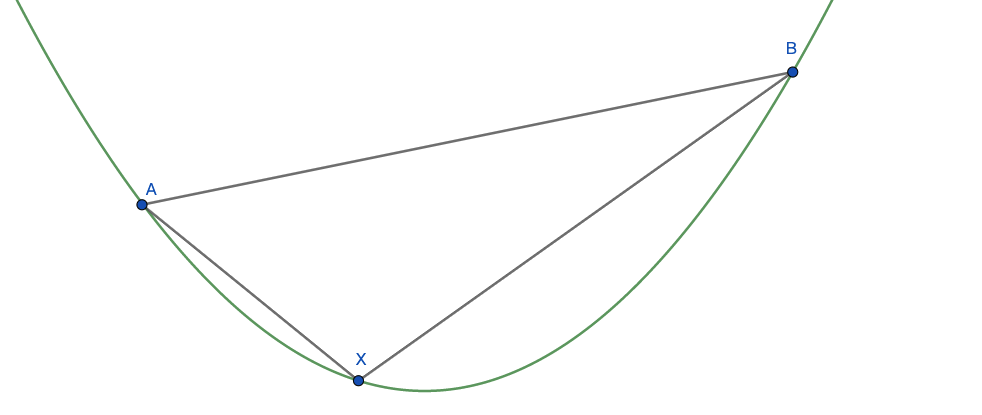
\includegraphics[width=0.6\textwidth]{./figure/fig1.png}
                \caption{sketch that illustrates this inequality \label{fig1}}
            \end{figure}
        \end{enumerate}
    \end{proof}
\end{problem}

\begin{problem}[3.7]
    Suppose $f : \mathbb{R}^n \to \mathbb{R}$ is convex with $\dom(f) = \mathbb{R}^n$. and bounded above on $\mathbb{R}^n$. Show that f is constant.

    \Answer Suppose $f$ is not constant. $\exists x, y$, s.t. $f(x) < f(y)$.
    \[g(t) = f(tx + (1 - t)y)\] is convex, $g(0) = f(y) > f(x) = g(1)$. We get
    \[g(0) \le \frac{t - 1}{t}g(1) + \frac{1}{t}g(t)\] for all $t > 1$, and
    \[g(t) \ge tg(0) - (t - 1)g(1) = g(1) + t(g(0) - g(1))\]
    so $g$ grows unboundedly as $t \to \infty$. This contradicts our assumption that $f$ is bounded. So $f$ is constant.
\end{problem}

\begin{problem}[3.16]
    For each of the following functions determine whether it is convex, concave, quasiconvex, or quasiconcave.(consider only convexity and concavity)
    \begin{enumerate}
        \item $f(x) = e^x - 1$ on $\mathbb{R}$.
        \item $f(x_1, x_2) = x_1x_2$ on $\mathbb{R}^2_{++}$.
        \item $f(x_1, x_2) = 1 / (x_1x_2)$ on $\mathbb{R}^2_{++}$.
        \item $f(x_1, x_2) = x_1/x_2$ on $\mathbb{R}^2_{++}$.
        \item $f(x_1, x_2) = x_1^2/x_2$ on $\mathbb{R}\times \mathbb{R}_{++}$.
        \item $f(x_1, x_2) = x_1^\alpha x_2^{1 - \alpha}$, where $0\le \alpha \le 1$, on $\mathbb{R}^2_{++}$.
    \end{enumerate}

    \Answer \text{}\begin{enumerate}
        \item $f^{\prime\prime}(x) = e^x > 0$, so $f$ is convex but not concave.
        \item $\nabla^2 f = \begin{pmatrix}
            0 & 1 \\
            1 & 0
        \end{pmatrix}$ is neither positive semidefinite nor negative semidefinite, so $f$ is neither convex nor concave.
        \item $\nabla^2f = \frac{1}{x_1^3x_2^3}\begin{pmatrix}
            2x_2^2 & x_1x_2 \\
            x_1x_2 & 2x_1^2
        \end{pmatrix} \succeq 0$, so $f$ is convex but not concave.
        \item $\nabla^2f = \frac{1}{x_2^3}\begin{pmatrix}
            0 & -x_2\\
            -x_2 & 2x_1
        \end{pmatrix}$ is neither positive semidefinite nor negative semidefinite, so $f$ is neither convex nor concave.
        \item $\nabla^2f = \frac{2}{x_2^3}\begin{pmatrix}
            x_2^2 & -x_1x_2 \\
            -x_1x_2 & x_1^2
        \end{pmatrix} \succeq 0$, so $f$ is convex but not concave.
        \item \begin{align*}    
            \nabla^2f &= \alpha(1 - \alpha)\begin{pmatrix}
                x_1^{\alpha - 2}x_2^{1 - \alpha} & -x_1^{\alpha - 1}x_2^{-\alpha}\\
                -x_1^{\alpha - 1}x_2^{-\alpha} & -x_1^\alpha x_2^{-\alpha - 1}
            \end{pmatrix}\\ 
            &=\alpha(1 - \alpha)x_1^{\alpha}x_2^{1 - \alpha}\begin{pmatrix}
                -1 / x_1^2 & 1 / x_1x_2 \\
                1 \ x_1x_2 & -1 / x_2^2
            \end{pmatrix}\\
            &=-\alpha(1 - \alpha)x_1^{\alpha}x_2^{1 - \alpha}\begin{pmatrix}
                1 / x_1 \\
                -1 / x_2
            \end{pmatrix}\begin{pmatrix}
                1 / x_1 & -1 / x_2
            \end{pmatrix}\\
            &\preceq 0
        \end{align*}
        so $f$ is concave but not convex.
    \end{enumerate}
\end{problem}

\begin{problem}[3.18]
    Adapt the proof of concavity of the log-determinant function in $\S 3.1.5$ to show the following.
    \begin{enumerate}
        \item $f(X) = \tr(X^{-1})$ is convex on $\dom(f) = \mathbb{R}^n_{++}$.
        \item $f(X) = (\operatorname{det} X)^{1 / n}$ is concave on $\dom(f) = \mathbb{R}^n_{++}$.
    \end{enumerate}

    \Answer \text{}
    \begin{enumerate}
        \item Define $g(t) = f(Z + tV)$, where $Z \succ 0$ and $V \in \mathbb{S}^n$. \begin{align*}
            g(t) &= \tr((Z + tV)^{-1})\\
            &= \tr(Z^{-1}(I + tZ^{-\frac{1}{2}}VZ^{-\frac{1}{2}})^{-1})\\
            &= \tr(Z^{-1} Q (I + t\Lambda)^{-1} Q^t)\\
            &= \tr(Q^tZ^{-1}Q(I + t\Lambda)^{-1})\\
            &= \sum_{i = 1}^n(Q^tZ^{-1}Q)_{ii}(1 + t\lambda_i)^{-1}
        \end{align*}
        We express $g$ as a positive weighted sum of convex functions $\frac{1}{1 + t\lambda_i}$, hence it is convex.
        \item Define $g(t) = f(Z + tV)$, where $Z \succ 0$ and $V \in \mathbb{S}^n$. \begin{align*}
            g(t) &= (\det(Z + tV))^{\frac{1}{n}}\\
            &= (\det(Z^{\frac{1}{2}}) \det(I + tZ^{-\frac{1}{2}}VZ^{-\frac{1}{2}}) \det(Z^{\frac{1}{2}}))^{\frac{1}{2}}\\ 
            &= (\det(Z))^{\frac{1}{n}}\left(\prod_{i = 1}^n(1 + t\lambda_i)\right)^{\frac{1}{n}}
        \end{align*}

        where $\lambda_i$ are the eigenvalues of $Z^{-\frac{1}{2}} V Z^{-\frac{1}{2}}$. We see that $g$ is a concave function of $t$ on $\left\{t \ | \ Z + tV \succ 0\right\}$, since $\det(Z) > 0$ and the geometric mean $(\prod_{i = 1}^nx_i)^{\frac{1}{n}}$ is concave on $\mathbb{R}_{++}^n$.
    \end{enumerate}
\end{problem}


\begin{problem}[3.27]
    \textit{Diagonal elements of Cholesky factor.} Each $X \in \mathbf{S}^n_{++}$ has a unique \textit{Cholesky factorization} $X = LL^T$, where $L$ is lower triangular, with $L_{ii} > 0$. Show that $L_{ii}$ is a concave function of $X$ (with domain $\mathbf{S}^n_{++}$).

    \textit{Hint.} $L_{ii}$ can be expressed as $L_{ii} = (w - z^tY^{-1}z)^{1 / 2}$, where\[\begin{bmatrix}
        Y & z \\
        z^T & w
    \end{bmatrix}\] is the leading $i \times i$ submatrix of $X$.

    \Answer $f(z, Y) = z^tY^{-1}z$ with $\dom(f) = \left\{(z, Y) | Y \succ 0\right\}$ is convex jointly in $z$ and $Y$. Notice that \[(z, Y, t) \in \operatorname{epi}(f) \quad \Longleftrightarrow \quad Y \succ 0, \quad\begin{bmatrix}
        Y & z \\
        z^t & T
    \end{bmatrix} \succeq 0\] so $\operatorname{epi}(f)$ is a convex set. Therefore, $w - z^tY^{-1}z$ is a concave function of $X$. Since the squareroot is an increasing concave function, it follows from the composition rules that $l_{kk} = (w - z^tY^{-1}z)^{\frac{1}{2}}$ is a concave function of $X$.
\end{problem}


\begin{problem}[3.31]
    \textit{Largest homogeneous und restimator.}Let $f$ be a convex function. Define the function $g$ as 
    \[g(x)=\inf _{\alpha>0} \frac{f(\alpha x)}{\alpha}\]
    \begin{enumerate}
        \item Show that $g$ is homogeneous ($g(tx) = tg(x)$ for all $t \ge 0$).
        \item Show that $g$ is the largest homogeneous underestimator of $f$: If $h$ is homogeneous and $h(x) \le f(x)$ for all $x$. then we have $h(x) \le g(x)$ for all $x$.
        \item show that $g$ is convex.
    \end{enumerate}

    \Answer \text{}\begin{enumerate}
        \item If $t = 0$, $g(tx) = g(0) = 0 = tg(x)$. If $t > 0$ \[g(t x)=\inf _{\alpha>0} \frac{f(\alpha t x)}{\alpha}=t \inf _{\alpha>0} \frac{f(\alpha t x)}{t \alpha}= tg(x) .\] so $\forall t \ge 0, g(tx) = tg(x)$.
        \item If $h$ is a homogeneous underestimator, then \[h(x) = \frac{h(\alpha x)}{\alpha} \le \frac{f(\alpha x)}{\alpha}\] for all $\alpha  > 0$, so $h(x) \le g(x)$.
        \item We can express $g$ as \[g(x) = \inf_{t > 0} tf(x / t) = \inf_{t > 0} h(x, t)\] where $h$ is the perspective function of $f$. We know $h$ is convex, so $g$ is convex.
    \end{enumerate}
\end{problem}

\begin{problem}[3.36]
    (\todo)
    Derive the conjugates of the following funetions.
    \begin{enumerate}
        \item \textit{Max function.} $f(x) = \max_{i = 1,\dots,n}x_i$ on $\mathbb{R}^n$.
        \item \textit{Saum of largest elements.} $f(x) = \sum_{i = 1}^r x_{[i]}$ on $\mathbb{R}^n$.
        \item \textit{Piecewise-linear function on} $\mathbb{R}$. $f(x) = \max_{i = 1, \dots, m}(a_ix + b_i)$ on $\mathbb{R}$. You can assume that the $a_i$ are sorted in increasing order, \textit{i.e.}, $a_1 \le \cdots \le a_m$, and that none of the functions $a_ix + b_i$: is redundant, \textit{i.e.}, for each $k$ there is at least one $x$ with $f(x) = a_kx + b_k$.
        \item \textit{Power function.} $f(x) = x^p$ on $\mathbb{R}_{++}^n$.
        \item \textit{Negative geometric mean.} $f(x) = -\left(\prod x_i\right)^{1 / n}$ on $\mathbb{R}_{++}^n$.
        \item \textit{Negative generalized logarithm for second-order cone.} $f(x, t) = -\log(t^2 - x^Tx)$ on $\left\{(x, t) \in \mathbb{R}^n\times \mathbb{R}\text{\ } |\text{\ } \|x\|_2 < t\right\}$.
    \end{enumerate}
\end{problem}

\begin{problem}[3.37]
    Show that the conjugate of $f(X) = \tr(X^{-1})$ with $\dom(f) = \mathbb{S}^n_{++}$ is given by\[f^*(Y) = -2\tr(-Y)^{\frac{1}{2}}, \quad \dom(f^*) = -\mathbb{S}_+^n\]

    \textit{Hint.} The gradient of $f$ is $\nabla f(X) = -X^{-2}$
    \Answer Suppose $Y$ has eigenvalue decomposition \[Y = Q\Lambda Q^t = \sum_{i = 1}^n \lambda_i q_i q_i^t\] with $\lambda_1 > 0$. Let $X = Q \diag(t, 1, \dots, 1)Q^t = tq_1q_1^t + \sum_{i = 2}^{n}q_iq_i^t$. We have \[\tr(XY) - \tr(X^{-1}) = t\lambda_1 + \sum_{i = 2}^n\lambda_i - 1 / t - (n - 1)\] which grows unboundedly as $t \to \infty$. Therefore $Y \notin \dom(f)^*$.

    Next, assume $Y \preceq 0$. If $Y \prec 0$, we can find the maximum of \[\tr(XY) - \tr(X^{-1})\] by setting the gradient equal to zero. We obtain $Y = -X^{-2}$, i.e., $X = (-Y)^{-1 / 2}$, and \[f^*(Y) = -2\tr(-Y)^{1 / 2}\]Finally we verify that this expression remains valid when $Y \preceq 0$, but $Y$ is singular. This follows from the fact that conjugate functions are always closed, i.e., have closed epigraphs.
\end{problem}

\section{Convex optimization problems}
\begin{problem}[4.1]
    Consider the optimization problem\[\begin{cases}
        \minimize \quad &f_0(x_1, x_2)\\
        \subject \quad &2x_1 + x_2 \ge 1\\
        &x_1 + 3x_2 \ge 1\\
        &x_1 \ge 0, \quad x_2 \ge 0
    \end{cases}\]
    Make a sketch of the feasible set. For each of the following objective functions, give the optimal set and the optimal value.
    \begin{enumerate}
        \item $f_0(x_1, x_2) = x_1 + x_2$
        \item $f_0(x_1, x_2) = -x_1 - x_2$
        \item $f_0(x_1, x_2) = x_1$
        \item $f_0(x_1, x_2) = \max\left\{x_1, x_2\right\}$
        \item $f_0(x_1, x_2) = x_1^2 + 9x_2^2$
    \end{enumerate}

    \Answer The feasible set is the convex hull of $(0, +\infty), (0, 1), (\frac{2}{5}, \frac{1}{5}), (1, 0), (+\infty, 0)$.
    \begin{enumerate}
        \item $x^* = (\frac{2}{5}, \frac{1}{5})$
        \item Unbounded below.
        \item $X = \left\{(0, x_2)\ |\ x_2 \ge 1\right\}$
        \item $x^* = (\frac{1}{3}, \frac{1}{3})$
        \item $x^* = (\frac{1}{2}, \frac{1}{6})$
    \end{enumerate}
\end{problem}

\begin{problem}[4.2]
    Consider the optimization problem\[\minimize \quad f_0(x) = -\sum_{i = 1}^m\log(b_i - a_i^tx)\] with domain $\dom(f_0) = \left\{x | Ax \prec b\right\}$, where $A \in \mathbb{R}^{m \times n}$(with rows $a_i^t$). We assume that $\dom(f_0)$ is nonempty.

    Prove the following facts(which include the results quoted without proof on page 141).
    \begin{enumerate}
        \item $\dom(f_0)$ is unbounded iff there exists a $v \neq 0$ with $Av \preceq 0$.
        \item $f_0$ is unbounded below iff there exists a $v$ with $Av \preceq 0, Av \neq 0$.\textit{Hint.}There exists a $v$ such that $Av \preceq 0, Av \neq 0$ iff there exists no $z \succ 0$ such that $A^tz = 0$. This follows from the theorem of alternatives in example 2.21, page 50.
        \item If $f_0$ is bounded below then its minimum is attained, i.e., there exists an $x$ that satisfies the optimality condition(4.23).
        \item The optimal set is affine: $X_{opt} = \left\{x^* + v\ |\ Av = 0\right\}$, where $x^*$ is any optimal point.
    \end{enumerate}
    \Answer \text{}\begin{enumerate}
        \item If such a $v$ exists, $\dom(f_0)$ is unbounded, since $x_0 + tv \in \dom(f_0)$ for all $t \ge 0$. Conversely, suppose $x^k$ is a sequence of points in $\dom(f_0)$ with $\|x^k\|_2 \to \infty$. Define $v^k = x^k / \|x^k\|_2$. The sequence has a convergent subsequence because $\|v^k\|_2 = 1$ for all $k$. Let $v$ be its limit. We have $\|v\|_2 = 1$ and, since $a_i^tv^k < b_i / \|x^k\|_2$ for all $k$, $a_i^tv \le 0$. Therefore $Av \preceq 0$ and $v \neq 0$.
        \item If there exists such a $v$, then $f_0$ is unbounded below. Let $j$ be an index with $a_j^tv < 0$. For $t \ge 0$, \begin{align*}
            f_0(x_0 + tv) &= -\sum_{i = 1}^m\log(b_i - a_i^tx_0 - ta_i^tv)\\
            & \le -\sum_{i \neq j}^m\log(b_i - a_i^tx_0) - \log(b_j - a_j^tx_0 - ta_j^tv)
        \end{align*} and the righthand side decreases without bound as $t$ increases.

        Conversely, suppose $f$ is unbounded below. Let $x^k$ be a sequence with $b - Ax^k \succ 0$, and $f_0(x^k) \to -\infty$. By convexity,\[f_0(x^k) \ge f_0(x_0) + \sum_{i = 1}^m\frac{1}{b_i - a_i^tx_0}a_i^t(x^k - x_0) = f_0(x_0) + m - \sum_{i = 1}^m\frac{b_i - a_i^tx^k}{b_i - a_i^tx_0}\] so if $f_0(x^k) \to -\infty$, we must have $\max_i(b_i - a_i^tx^k) \to \infty$.

        Suppose there exists a $z$ with $z \succ 0$, $A^tz = 0$. Then \[z^tb = z^t(b - Ax^k) \ge z_i\max_{i}(b_i - a_i^tx^k) \to \infty\]
        We have reached a contradiction, and conclude that there is no such $z$. Using the theorem of alternatives, there must be a $v$ with $Av \preceq 0, Av \neq 0$.
        \item We can assume that $\rank(A) = n$.
        
        If $\dom(f_0)$ is bounded, then the result follows from the fact that the sublevel sets of $f_0$ are closed.

        If $\dom(f_0)$ is unbounded, let $v$ be a direction in which it is unbounded, i.e., $v \neq 0, Av \preceq 0$. Since $\rank(A) = 0$, we must have $Av \neq 0$, but this implies $f_0$ is unbounded. We conclude that if $\rank(A) = n$, then $f_0$ is bounded below iff its domain is bounded, and therefore its minimum is attained.
        \item We can limit $\rank(A) = n$. We show that $f_0$ has at most one optimal point. The Hessian of $f_0$ at $x$ is \[\nabla^2f(x) = A^t\diag(d)A, \quad d_i = \frac{1}{(b_i - a_i^tx)^2}, \ i = 1, \dots, m\] which is positive definite if $\rank(A) = n$, i.e., $f_0$ is strictly convex. Therefore the optimal point, if it exists, is unique. 
    \end{enumerate}
\end{problem}

\begin{problem}[4.3]
    Prove that $x^* = \left(1, \frac{1}{2}, -1\right)$ is optimal for the optimization problem\[\begin{cases}
        \minimize \quad &\frac{1}{2}x^tPx + q^tx + r\\
        \subject \quad & -1 \le x_i \le 1, \quad i = 1, 2, 3
    \end{cases}\] where \[P = \begin{bmatrix}
        13 & 12 & -2\\
        12 & 17 & 6\\
        -2 & 6 & 12\\
    \end{bmatrix}, \quad q = \begin{bmatrix}
        -22.0 \\ -14.5 \\ 13.0
    \end{bmatrix}, \quad r = 1\]
    \Answer $\nabla f_0(x^*) = (-1, 0, 2)$. Therefore the optimality condition is that $\nabla f_0(x^*)^t(y - x) = -(y_1 - 1) + 2(y_2 + 1) \ge 0$ for all $y$ satisfying $-1 \le y_i \le 1$.
\end{problem}

\begin{problem}[4.8]
    Some simple LPs. Give an explicit solution of each of the following LPs.
    \begin{enumerate}
        \item Minimizing a linear function over an affne set.\[\begin{cases}
            \minimize \quad & c^tx \\
            \subject \quad &Ax = b
        \end{cases}\]
        \item Minimizing a linear function over a halfspace \[\begin{cases}
            \minimize \quad & c^tx \\
            \subject \quad &a^tx \le b
        \end{cases}\] where $a \neq 0$.
        \item Minimizing a linear function over a rectangle.\[\begin{cases}
            \minimize \quad & c^tx \\
            \subject \quad & l \preceq x \preceq u
        \end{cases}\] where $l$ and $u$ satisfy $l \preceq u$.
        \item Minimizing a linear function over the probability simplex.\[\begin{cases}
            \minimize \quad & c^tx \\
            \subject \quad & \textbf{1}^tx = 1, \quad x \succeq 0
        \end{cases}\]
        What happens if the equality constraint is replaced by an inequality $\textbf{1}^tx \le 1$? We can interpret this LP as a simple portfolio optimization problem. The vector $x$ represents the allocation of our total budget over different assets, with $x_i$ the fraction invested in asset $i$. The return of each investment is fixed and given by $-c_i$, so our total return (which we want to maximize) is $-c^tx$. If we replace the budget constraint $\textbf{1}^tx = 1$ with an inequality $\textbf{1}^tx \le 1$, we have the option of not investing a portion of the total budget.
        \item Minimizing a linear function over a unit box with a total budget constraint.\[\begin{cases}
            \minimize \quad & c^tx \\
            \subject \quad &\textbf{1}^tx = \alpha, \quad 0 \preceq x \preceq \textbf{1}
        \end{cases}\] where $\alpha$ is an integer between 0 and $n$. What happens if $\alpha$ is not an integer (but satisfies $0 \le \alpha \le n$)? What if we change the equality to an inequality $\textbf{1}^tx \le \alpha$?
        \item Minimizing a linear function over a unit box with a weighted budget constraint.\[\begin{cases}
            \minimize \quad & c^tx \\
            \subject \quad &d^tx = \alpha, \quad 0 \preceq x \preceq \textbf{1}
        \end{cases}\] with $d \succ 0$, and $0 \le \alpha \le \textbf{1}^td$.
    \end{enumerate}
    \Answer \text{} \begin{enumerate}
        \item \begin{itemize}
            \item If $b \notin \mathcal{R}(A)$, the optimal value is $\infty$.
            \item If $c$ is orthogonal to the nullspace of $A$. $c = A^t\lambda + \hat{c}, A\hat{c} = 0$. So $c^tx = \lambda^tAx + \hat{c}^tx = \lambda^tb$. The optimal value is $\lambda^tb$.
            \item If $c$ is not in the range of $A^t(\hat{c}\neq 0)$, the problem is unbounded$(p^* = -\infty)$. To verify this, note that $x = x_0 - t\hat{c}$ is feasible for all $t$, $t \to \infty$, than target $\to $ unbounded.
        \end{itemize}
        In summary, \[p^* = \begin{cases}
            +\infty \quad &b \notin \mathcal{R}(A)\\
            \lambda^tb\quad &c = A^t\lambda \text{ for some } \lambda\\
            -\infty \quad &\text{otherwise}
        \end{cases}\]
        \item Let $c = a\lambda + \hat{c}$, with $a^t\hat{c} = 0$.\begin{itemize}
            \item If $\lambda > 0$, the problem is unbounded below. Choose $x = -ta$, and let $t \to \infty$:\[c^tx = -tc^ta = -t\lambda a^ta \to -\infty\] and \[a^tx - b = -ta^ta - b \le 0\] for large $t$, so $x$ is feasible for large $t$. 
            \item If $\hat{c} \neq 0$, the problem is unbounded blow. Choose $x = ba - t\hat{c}$ and $t \to \infty$.
            \item If $c = a\lambda$ for some $\lambda \le 0$, the optimal value is $c^tab = \lambda b$
        \end{itemize}
        In summary, the optimal value is \[*p = \begin{cases}
            \lambda b \quad &c = a\lambda \text{ for some } \lambda \le 0\\
            -\infty \quad &\text{otherwise}
        \end{cases}\]
        \item The optimal $x_i^*$ minimizes $c_ix_i$ subject to the constraint $l_i \le x_i \le u_i$. If $c_i > 0$, then $x_i^* = l_i$; if $c_i < 0$, then $x_i^* = u_i$; if $c_i = 0$, then any $x_i$ in the interval $[l_i, u_i]$ is optimal. Therefore, the optimal value of the problem is \[p^* = l^tc^+ + u^tc^-\] where $c_i^+ = \max\left\{c_i, 0\right\}$ and $c_i^- = \max\left\{-c_i, 0\right\}$.
        \item $c^tx = c_{\min}$, $x_i = 0$ if $c_i > c_{\min}$.
        \item Suppose $c_i$ is sorted, the optimal value if $p^* = c_1 + c_2 + \cdots + c_{\left \lfloor \alpha \right \rfloor } + c_{1 + \left \lfloor \alpha \right \rfloor }(\alpha - \left \lfloor \alpha \right \rfloor )$. 
        \item Suppose that \[\frac{c_{1}}{d_{1}} \leq \frac{c_{2}}{d_{2}} \leq \cdots \leq \frac{c_{n}}{d_{n}}\] To minimize the objective, we choose \[y_1 = d_1, \quad y_2 = d_2, \quad \cdots, \quad y_k = d_k\] where $k = \max\left\{i \in \left\{1, \dots, n\right\} |\ d_1 + \cdot + d_i \le \alpha\right\}$ (and $k = 0$ if $d_1 > \alpha$). In trems of the original variables.\[x_{1}=\cdots=x_{k}=1, \quad x_{k+1}=\left(\alpha-\left(d_{1}+\cdots+d_{k}\right)\right) / d_{k+1}, \quad x_{k+2}=\cdots=x_{n}=0\]
    \end{enumerate}
\end{problem}

\begin{problem}[4.9]
    Square LP. Consider the LP \[\begin{cases}
        \minimize \quad &c^tx \\
        \subject \quad &Ax \preceq b
    \end{cases}\] with $A$ square and nonsingular. Show that optimal value is given by \[p^* = \begin{cases}
        c^tA^{-1}b \quad &A^{-t}c \preceq 0\\
        -\infty \quad &\text{otherwise}
    \end{cases}\]
    \Answer $y = Ax$. We get \[\begin{cases}
        \minimize\quad &c^tA^{-1}y\\
        \subject\quad &y \preceq b
    \end{cases}\] If $A^{-t}c \preceq 0$, the optimal solution is $y = b$, with $p^* = c^tA^{-1}b$. Otherwise, the LP is unbounded below.
\end{problem}

\begin{problem}[4.15]
    Relaration of Boolean LP. In a Boolean linear program, the variable $x$ is constrained to have components equal to zero or one:\begin{equation}\label{eq1}
        \begin{cases}
            \minimize \quad &c^tx \\
            \subject \quad &Ax \preceq b\\
            &x_i \in \left\{0, 1\right\}, \quad i = 1, \dots, n
        \end{cases}
    \end{equation}

    In general, such problems are very difficult to solve, even though the feasible set is finite (containing at most $2^n$ points).

    In a general method called relawation, the constraint that $x_i$ be zero or one is replaced with the linear inequalities $0 \le x_i \le 1$:\begin{equation}\label{eq2}
        \begin{cases}
            \minimize \quad &c^tx \\
            \subject \quad &Ax \preceq b\\
            &0 \le x_i \le 1, \quad i = 1, \dots, n
        \end{cases}
    \end{equation}

    We refer to this problem as the LP(\ref{eq1}) relaration of the Boolean LP. The LP relaxation is far easier to solve than the original Boolean LP.
    \begin{enumerate}
        \item Show that the optimal value of the LP relaxation(\ref{eq2}) is a lower bound on the optimal value of the Boolean LP (\ref{eq1}). What can you say about the Boolean LP if the LP relaxation is infeasible?
        \item It sometimes happens that the LP relaxation has a solution with $x_i \in \left\{0, 1\right\}$. What can you say in this case?
    \end{enumerate}
    \Answer \text{}\begin{enumerate}
        \item The feasible set of the relaxation includes the feasible set of the Boolean LP. It follows that the Boolean LP is infeasible if the relaxation is infeasible, and that the optimal value of the relaxation is less than or equal to the optimal value of the Boolean LP.
        \item The optimal solution of the relaxation is also optimal for the Boolean LP.
    \end{enumerate}
\end{problem}

\begin{problem}[4.21]
    Some simple QCQPs. Give an explicit solution of each of the following QCQPs.
    \begin{enumerate}
        \item Minimizing a linear function over an ellipsoid centered at the origin.\[\begin{cases}
            \minimize \quad &c^tx\\
            \subject \quad &x^tAx \le 1
        \end{cases}\]
        where $A \in \mathbb{S}_{++}^n$ and $c \neq 0$. What is the solution if the problem is not convex($A \notin \mathbb{S}_+^n$)?
        \item Minimizing a linear function over an ellipsoid.\[\begin{cases}
            \minimize \quad &c^tx \\
            \subject \quad &(x - x_c)^t A (x - x_c) \le 1
        \end{cases}\] where $A \in \mathbb{S}_{++}^n$ and $c \neq 0$.
        \item Minimizing a quadratic form over an ellipsoid centered at the origin. \[\begin{cases}
            \minimize \quad &x^tBx \\
            \subject \quad &x^tAx \le 1
        \end{cases}\] where $A \in \mathbb{S}_{++}^n$ and $B \in \mathbb{S}_+^n$. Also consider the nonconvex extension with $B \notin \mathbb{S}_+^n$.
    \end{enumerate}
    \Answer \text{}\begin{enumerate}
        \item If $A \succ 0$, the solution is \[x^{\star}=-\frac{1}{\sqrt{c^{T} A^{-1} c}} A^{-1} c, \quad p^{\star}=-\left\|A^{-1 / 2} c\right\|_{2}=-\sqrt{c^{T} A^{-1} c}\]
        We make a change of variables $y = A^{1 / 2}x$, and write $\tilde{c} = A^{-1 / 2}c$. With this new variable the optimization problem becomes\[\begin{cases}
            \minimize \quad &\tilde{c}^ty\\
            \subject \quad &y^ty \le 1
        \end{cases}\]The answer is $y^* = -\tilde{c} / \|\tilde{c}\|_2$. \[A = Q\diag(\lambda)Q^t = \sum_{i = 1}^n\lambda_iq_iq_i^t\]
        We define $y = Qx, b = Qc$, and express the problem as \[\begin{cases}
            \minimize \quad &\sum_{i = 1}b_iy_i\\
            \subject\quad &\sum_{i = 1}^n\lambda_iy_i \le 1
        \end{cases}\]If $\lambda_i > 0$ for all $i$, the problem reduces to the case we already discussed. Otherwise, we can distinguish several cases.\begin{itemize}
            \item $\lambda_n < 0$. The problem is unbounded below. Let $y_n \to \infty$, we can make any point feasible.
            \item $\lambda_n = 0$. If for some $i$, $b_i \neq 0$ and $\lambda_i = 0$, the problem is unbounded below.
            \item $\lambda_n = 0$, and $b_i = 0$ for all $i$ with $\lambda_i = 0$. In this case we can reduce the problem to a smaller one with all $\lambda_i > 0$. 
        \end{itemize}
        \item $y = A^{1 / 2}(x - x_c), x = A^{-1 / 2}y + x_c$, and consider the problem\[\begin{cases}
            \minimize \quad &c^tA^{-1 / 2}y + c^tx_c\\
            \subject\quad &y^ty \le 1
        \end{cases}\] The solution is \[y^{\star}=-\left(1 /\left\|A^{-1 / 2} c\right\|_{2}\right) A^{-1 / 2} c, \quad x^{\star}=x_{c}-\left(1 /\left\|A^{-1 / 2} c\right\|_{2}\right) A^{-1} c .\]
        \item If $B \succ 0$, then the optimal value is zero.
        
        The smallest eigenvalue of $B \in \mathbb{S}^n$, can be characterized as\[\lambda_{\min}(B) = \inf_{x^tx = 1}x^tBx\]
        which equals to the problem \[\begin{cases}
            \minimize \quad &y^tA^{-1/2}BA^{-1/2}y\\
            \subject \quad &y^ty \le 1
        \end{cases}\] the optimal value is $\lambda_{\min}(A^{-1/2}BA^{-1/2})$
        
        To summarize, the optimal value is \[p^{\star}=\begin{cases}
            \lambda_{\min }\left(A^{-1 / 2} B A^{-1 / 2}\right) & \lambda_{\min }\left(A^{-1 / 2} B A^{-1 / 2}\right) \leq 0 \\
            0 & \qotherwise 
        \end{cases}\]
    \end{enumerate}
\end{problem}

\begin{problem}[4.22]
    Consider the QCQP\[\begin{cases}
        \minimize \quad &\frac{1}{2} x^tPx + q^tx + r\\
        \subject \quad &x^tx \le 1
    \end{cases}\]
    with $P \in \mathbb{S}_{++}^n$. Show that $x^* = -(P + \lambda I)^{-1}q$ where $\lambda = \max\left\{0, \bar{\lambda}\right\}$ and $\bar{\lambda}$ is the largest solution of the nonlinear equation \[q^t(P + \lambda I)^{-2}q = 1\]
    \Answer $x$ is optimal if and only if $x^tx < 1, Px + q = 0 \qor x^tx = 1, Px + q = -\lambda x$ for some $\lambda \ge 0$. If $\norm{P^{-1}q}_2 \le 1$, it is optimal. Otherwise, $\norm{x}_2 = 1 \qand (P + \lambda)x = -q$ for some $\lambda \ge 0$. $f(\lambda) = \norm{(P + \lambda)^{-1}q}_2^2 = \sum_{i = 1}^n \frac{q_i^2}{(\lambda + \lambda_i)^2}$ where $\lambda_i > 0$ are the eigenvalues of $P$. The nonlinear equation $f(\lambda) = 1$ has exactly one nonnegative solution $\bar{\lambda}$. The optimal solution is $x^* = -(P + \bar{\lambda}I)^{-1}q$.
\end{problem}

\section{Duality}
\begin{problem}[5.3]
    Problems with one inequality constraint. Express the dual problem of\[\begin{cases}
        \minimize \quad &c^tx \\
        \subject \quad &f(x) \le 0
    \end{cases}\] with $c \neq 0$, in terms of the conjugate $f^*$. Explain why the problem you give is convex. We do not assume $f$ is convex.
    \Answer For $\lambda = 0, g(\lambda) = \inf c^tx = -\infty$. For $\lambda > 0$, $g(\lambda) = \inf (c^tx + \lambda f(x)) = \lambda \inf ((c / \lambda)^tx + \lambda f(x) = -\lambda f_1^*(-c/\lambda)$. The dual problem is \[\begin{cases}
        \minimize\quad &-\lambda f_1^*(-c/\lambda)\\
        \subject\quad &\lambda \ge 0
    \end{cases}\]
\end{problem}

\begin{problem}[5.5]
    Dual of general LP. Find the dual function of the LP\[\begin{cases}
        \minimize \quad &c^tx\\
        \subject \quad &Gx \preceq h\\
        &Ax = b
    \end{cases}\] Give the dual problem, and make the implicit equality constraints explicit.
    \Answer \text{}\begin{enumerate}
        \item The Lagrangian is \[L(x, \lambda, \mu) = \left(c^{T}+\lambda^{T} G+\mu^{T} A\right) x-h \lambda^{T}-\mu^{T} b\] which is an affine function of $x$. It follows that the dual function is given by \[g(\lambda, \mu) = \inf_{x} L(x, \lambda, \mu) = \begin{cases}
            -\lambda^t h-\mu^t b & c+G^t \lambda+A^t \mu=0 \\
            -\infty & \qotherwise
        \end{cases}\]
        \item The dual problem is\[\begin{cases}
            \maximize \quad &g(\lambda, \mu)\\
            \subject \quad &\lambda \succeq 0
        \end{cases}\]After making the implicit constraints explicit, we obtain\[\begin{cases}
            \maximize \quad &-\lambda^th - \mu^tb\\
            \subject \quad &c + G^t\lambda + A^t\mu = 0\\
            &\lambda \ge 0
        \end{cases}\]
    \end{enumerate}
\end{problem}

\begin{problem}[5.11]
    Derive a dual problem for \[\minimize \quad \sum_{i = 1}^N \|A_ix + b_i\|_2 + \frac{1}{2}\|x - x_0\|_2^2\] The problem data are $A_i \in \mathbb{R}^{m_i \times n}$; $b_i \in \mathbb{R}^{m_i}$. and $x_0 \in \mathbb{R}^n$. First introduce new variables $y_i \in \mathbb{R}^{m_i}$ and equality constraints $y_i = A_ix + b_i$.
    \Answer The Lagrangian is\[L\left(x, z_{1}, \ldots, z_{N}\right)=\sum_{i=1}^{N}\left\|y_{i}\right\|_{2}+\frac{1}{2}\left\|x-x_{0}\right\|_{2}^{2}-\sum_{i=1}^{N} z_{i}^{t}\left(y_{i}-A_{i} x-b_{i}\right)\]We frst minimize over $y_i$.\[\inf _{y_{i}}\left(\left\|y_{i}\right\|_{2}+z_{i}^{T} y_{i}\right)=\left\{\begin{array}{ll}
        0 & \left\|z_{i}\right\|_{2} \leq 1 \\
        -\infty & \text { otherwise }
    \end{array}\right.\]
    We can minimize over $x$ by setting the gradient with respect to $x$ equal to zero. \[x = x_0 + \sum_{i = 1}^NA_i^tz\]
    Substituting in the Lagrangian gives the dual function \[g\left(z_{1}, \ldots, z_{N}\right)=\left\{\begin{array}{ll}
        \sum_{i=1}^{N}\left(A_{i} x_{0}+b_{i}\right)^{t} z_{i}-\frac{1}{2}\left\|\sum_{i=1}^{N} A_{i}^{t} z_{i}\right\|_{2}^{2} & \left\|z_{i}\right\|_{2} \leq 1, \quad i=1, \ldots, N \\
        \text { otherwise }
        \end{array}\right.\]
    The dual problem is\[\begin{cases}
        \maximize\quad &\sum_{i=1}^{N}\left(A_{i} x_{0}+b_{i}\right)^{t} z_{i} - \frac{1}{2}\norm{\sum_{i=1}^{N} A_{i}^{t} z_{i}}^2\\
        \subject \quad &\norm{z_i}_2 \le 1, i = 1, \dots, N
    \end{cases}\]
\end{problem}

\begin{problem}[5.12]
    Analytic centering. Derive a dual problem for\[\minimize \quad -\sum_{i = 1}^m \log(b_i - a_i^tx)\] with domain $\left\{x\ |\ a_i^tx < b_i, i = 1, \dots, m\right\}$. First introduce new variables $y_i$ and equality constraints $y_i = b_i - a_i^tx$.

    (The solution of this problem is called the analytic center of the linear inequalities $a_i^tx \le b_i, i = 1, \dots, m$. Analytic centers have geometric applications (see \S8.5.3), and play an important role in barrier methods (see chapter 11).)
    \Answer We derive the dual of the problem\[\begin{cases}
        \minimize \quad &-\sum_{i = 1}^m\log y_i\\
        \subject \quad &y = b - Ax
    \end{cases}\]where $A \in \mathbb{R}^{m \times n}$ has $a_i^t$ as its $i$th row. The Lagrangian is\[L(x, y, \mu)=-\sum_{i=1}^{m} \log y_{i}+\mu^{T}(y-b+A x)\] and the dual function is \[g(\mu) = \inf_{x, y}\left(-\sum_{i = 1}^m\log y_i + \mu^t(y - b + Ax)\right)\] The term $\mu^tAx$ is unbounded below as a function of $x$ unless $A^t\mu = 0$. The terms in y are unbounded below if $\mu \nsucc$, and achieve their minimum for $y_i = 1 / \mu_i$ otherwise. We therefore find the dual function\[g(\mu)=\left\{\begin{array}{lll}
        \sum_{i=1}^{m} \log \nu_{i}+m-b^{T} \mu & A^{T} \mu=0, & \mu \succ 0 \\
        -\infty & \text { otherwise } &
        \end{array}\right.\] and the dual problem \[\begin{cases}
            \maximize \quad &\sum_{i = 1}^m\log \mu_i - b^t\mu + m\\
            \subject \quad &A^t\mu = 0
        \end{cases}\]
\end{problem}

\begin{problem}[5.21]
    A conven problem in which strong duality fails. Consider the optimization problem\[\begin{cases}
        \minimize\quad &e^{-x}\\
        \subject\quad &x^2/y\le 0
    \end{cases}\]with variables $x$ and $y$, and domain $\mathcal{D} = \left\{(x, y)\mid y > 0\right\}$.
    \begin{enumerate}
        \item Verify that this is a convex optimization problem. Find the optimal value.
        \item Give the Lagrange dual problem, and find the optimal solution $\lambda^*$ and optimal value $d^*$ of the dual problem. What is the optimal duality gap?
        \item Does Slater's condition hold for this problem?
        \item What is the optimal value $p^*(u)$ of the perturbed problem\[\begin{cases}
            \minimize\quad &e^{-x}\\
            \subject\quad &x^2/y \le u
        \end{cases}\] as a function of $u$? Verify that the global sensitivity inequality\[p^*(u) \ge p^*(0) - \lambda^*u\] does not hold.
    \end{enumerate}
    \Answer \text{}\begin{enumerate}
        \item $p^* = 1$.
        \item The Lagrangian is $L(x, y, \lambda) = e^{-x} + \lambda x^2/y$. The dual function if \[g(\lambda)=\inf _{x, y>0}\left(e^{-x}+\lambda x^{2} / y\right)=\left\{\begin{array}{ll}
            0 & \lambda \geq 0 \\
            -\infty & \lambda<0
        \end{array}\right.\] so we can write the dual problem as \[\begin{cases}
            \minimize\quad &0\\
            \subject\quad & \lambda \ge 0
        \end{cases}\] with optimal value $d^* = 0$. The optimal duality gap is $p^* - d^* = 1$.
        \item Slater's condition is not satisfied.
        \item $p^*(u) = 1\text{ if } u = 0, p^*(u) = 0\text{ if } u > 0 \text{ and } p^*(u) = \infty \text{ if } u < 0$.
    \end{enumerate}
\end{problem}

\begin{problem}[5.26]
    Consider the QCQP\[\begin{cases}
        \minimize\quad &x_1^2 + x_2^2\\
        \subject\quad &(x_1 - 1)^2 + (x_2 - 1)^2 \le 1\\
        &(x_1 - 1)^2 + (x_2 + 1)^2 \le 1
    \end{cases}\] with variable $x \in \mathbb{R}^2$.
    \begin{enumerate}
        \item Sketch the feasible set and level sets of the objective. Find the optimal point $x^*$ and optimal value $p^*$.
        \item Give the KKT conditions. Do there exist Lagrange multipliers $\lambda_1^*$ and $\lambda_2^*$ that prove that $x^*$ is optimal?
        \item Derive and solve the Lagrange dual problem. Does strong duality hold?
    \end{enumerate}
    \Answer \text{}\begin{enumerate}
        \item The figure \ref{fig2} shows the feasible set(the intersection of the two shaded disks) and some contour lines of the objective function. There is only one feasible point $(1,0)$, and we have $p^* = 1$.\begin{figure}[htbp]
            \centering
            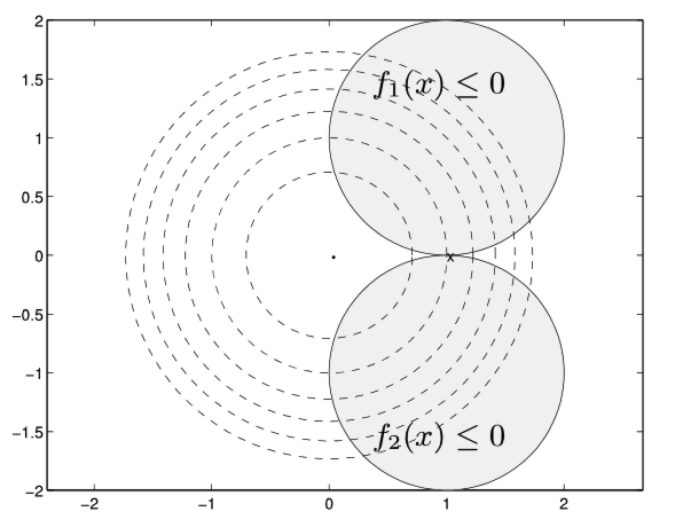
\includegraphics[width=0.4\textwidth]{./figure/fig2.png}
            \caption{the feasible set \label{fig2}}
          \end{figure}
          \item The KKT conditions are\[\begin{array}{c}
            \left(x_{1}-1\right)^{2}+\left(x_{2}-1\right)^{2} \leq 1, \quad\left(x_{1}-1\right)^{2}+\left(x_{2}+1\right)^{2} \leq 1, \\
            \lambda_{1} \geq 0, \quad \lambda_{2} \geq 0 \\
            2 x_{1}+2 \lambda_{1}\left(x_{1}-1\right)+2 \lambda_{2}\left(x_{1}-1\right)=0 \\
            2 x_{2}+2 \lambda_{1}\left(x_{2}-1\right)+2 \lambda_{2}\left(x_{2}+1\right)=0 \\
            \lambda_{1}\left(\left(x_{1}-1\right)^{2}+\left(x_{2}-1\right)^{2}-1\right)=\lambda_{2}\left(\left(x_{1}-1\right)^{2}+\left(x_{2}+1\right)^{2}-1\right)=0 .
            \end{array}\] At $x = (1,0)$, these conditions reduce to\[\lambda_{1} \geq 0, \quad \lambda_{2} \geq 0, \quad 2=0, \quad-2 \lambda_{1}+2 \lambda_{2}=0\] which have no solution.
        \item The Lagrange dual function is given by\[g\left(\lambda_{1}, \lambda_{2}\right)=\inf _{x_{1}, x_{2}} L\left(x_{1}, x_{2}, \lambda_{1}, \lambda_{2}\right)\] where \begin{align*}
            &L\left(x_{1}, x_{2}, \lambda_{1}, \lambda_{2}\right) \\
            =&x_{1}^{2}+x_{2}^{2}+\lambda_{1}\left(\left(x_{1}-1\right)^{2}+\left(x_{2}-1\right)^{2}-1\right)+\lambda_{2}\left(\left(x_{1}-1\right)^{2}+\left(x_{2}+1\right)^{2}-1\right) \\
            =&\left(1+\lambda_{1}+\lambda_{2}\right) x_{1}^{2}+\left(1+\lambda_{1}+\lambda_{2}\right) x_{2}^{2}-2\left(\lambda_{1}+\lambda_{2}\right) x_{1}-2\left(\lambda_{1}-\lambda_{2}\right) x_{2}+\lambda_{1}+\lambda_{2}
        \end{align*}
        L reaches its minimum for \[x_{1}=\frac{\lambda_{1}+\lambda_{2}}{1+\lambda_{1}+\lambda_{2}}, \quad x_{2}=\frac{\lambda_{1}-\lambda_{2}}{1+\lambda_{1}+\lambda_{2}}\] and we find \[g\left(\lambda_{1}, \lambda_{2}\right)=\left\{\begin{array}{ll}
            -\frac{\left(\lambda_{1}+\lambda_{2}\right)^{2}+\left(\lambda_{1}-\lambda_{2}\right)^{2}}{1+\lambda_{1}+\lambda_{2}}+\lambda_{1}+\lambda_{2} & 1+\lambda_{1}+\lambda_{2} \geq 0 \\
            -\infty & \text { otherwise }
        \end{array}\right.\]
        Since $g$ is symmetric, the optimum occurs with $\lambda_1 = \lambda_2$. The dual function then simplifies to\[g(\lambda_1, \lambda_2) = \frac{2\lambda_1}{2\lambda_1 + 1}\] 
        We see that $g(\lambda_1, \lambda_2)$ tends to $1$ as $\lambda_1 \to \infty$. We have $d^* = p^* = 1$, but the dual optimum is not attained.

        In this example, the KKT conditions fail because the dual optimum is not attained.
    \end{enumerate}
\end{problem}

\begin{problem}[5.27]
    Equality constrained least-squares. Consider the equality constrained least-squares problem\[\begin{cases}
        \minimize\quad &\norm{Ax - b}_2^2\\
        \subject\quad &Gx = h
    \end{cases}\] where $A \in \mathbb{R}^{m \times n}$ with $\rank(A) = n$, and $G \in \mathbb{R}^{p\times n}$ with $\rank(G) = p$.

    Give the KKT conditions, and derive expressions for the primal solution $x^*$ and the dual solution $\nu^*$.
    \Answer \text{}\begin{enumerate}
        \item The Lagrangian is \[\begin{aligned}
            L(x, \nu) &=\|A x-b\|_{2}^{2}+\nu^{T}(G x-h) \\
            &=x^{T} A^{T} A x+\left(G^{T} \nu-2 A^{T} b\right)^{T} x-\nu^{T} h,
        \end{aligned}\] with minimizer $x = -(1 / 2)(A^tA)^{-1}(G^t\nu - 2A^tb)$. The dual function is\[g(\nu)=-(1 / 4)\left(G^{T} \nu-2 A^{T} b\right)^{T}\left(A^{T} A\right)^{-1}\left(G^{T} \nu-2 A^{T} b\right)-\nu^{T} h\]
        \item The optimality conditions are\[2A^t(Ax^* - b) + G^t\nu^* = 0, \quad Gx^* = h\]
        \item From the first equation, \[x^{\star}=\left(A^{t} A\right)^{-1}\left(A^{t} b-(1 / 2) G^{t} \nu^{\star}\right)\] Plugging this expression for $x^*$ into the second equation gives\[G\left(A^{t} A\right)^{-1} A^{t} b-(1 / 2) G\left(A^{t} A\right)^{-1} G^{T} \nu^{\star}=h\] Substituting in the first expression gives an analytical expression for $x^*$.
    \end{enumerate}
\end{problem}

\begin{problem}[5.29]
    The problem\[\begin{cases}
        \minimize\quad &-3 x_{1}^{2}+x_{2}^{2}+2 x_{3}^{2}+2\left(x_{1}+x_{2}+x_{3}\right)\\
        \subject\quad &x_{1}^{2}+x_{2}^{2}+x_{3}^{2}=1 
    \end{cases}\]is a special case of (5.32), so strong duality holds even though the problem is not convex. Derive the KKT conditions. Find all solutions $x, \nu$ that satisfy the KKT conditions. Which pair corresponds to the optimum?
    \Answer \text{}\begin{enumerate}
        \item The KKT conditions are\[x_{1}^{2}+x_{2}^{2}+x_{3}^{2}=1, \quad(-3+\nu) x_{1}+1=0, \quad(1+\nu) x_{2}+1=0, \quad(2+\nu) x_{3}+1=0\]
        \item From the KKT conditions  $\nu \notin \left\{2, -1, 3\right\}$. We can therefore eliminate $x$ and reduce the KKT conditions to a nonlinear equation in $\nu$:\[\frac{1}{(-3 + \nu)} + \frac{1}{(1 + \nu)} + \frac{1}{(2 + \nu)} = 1\] The lefthand side is plotted in the figure. \begin{figure}[htbp]
            \centering
            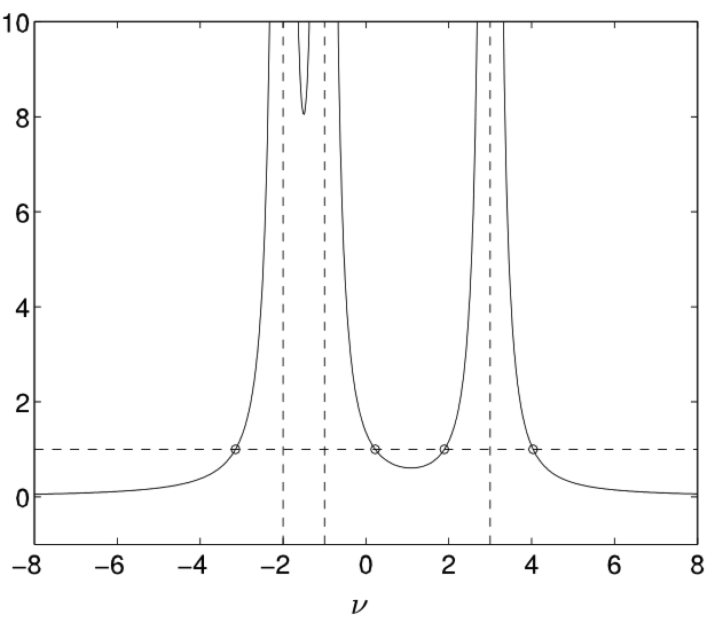
\includegraphics[width=0.5\textwidth]{./figure/fig3.png}
            \caption{the lefthand side \label{fig3}}
        \end{figure}
        There are four solutions:\[\nu=-3.15, \quad \nu=0.22, \quad \nu=1.89, \quad \nu=4.04\] corresponding to \begin{align*}
            x=(0.16,0.47,-0.87),\quad & x=(0.36,-0.82,0.45) \\
            x=(0.90,-0.35,0.26),\quad & x=(-0.97,-0.20,0.17)
        \end{align*}
        \item $\nu^*$ is the largest of the four values: $\nu^* = 4.0352$. This can be seen several ways. The simplest way is to compare the objective values of the four solutions $x$, which are \[f_{0}(x)=1.17, \quad f_{0}(x)=0.67, \quad f_{0}(x)=-0.56, \quad f_{0}(x)=-4.70\]We can also evaluate the dual objective at the four candidate values for $\nu$. Finally we can note that we must have\[\nabla^{2} f_{0}\left(x^{\star}\right)+\nu^{\star} \nabla^{2} f_{1}^{\star}\left(x^{\star}\right) \succeq 0\] because $x^*$ is a minimizer of $L(x, \nu^*)$. In other words \[\begin{bmatrix}
            -3 & 0 & 0\\
            0 & 1 & 0\\
            0 & 0 & 2
        \end{bmatrix} + \nu^*\begin{bmatrix}
            1 & 0 & 0\\
            0 & 1 & 0\\
            0 & 0 & 1
        \end{bmatrix} \succeq 0\] and therefore $\nu^* \ge 3$.
    \end{enumerate}
\end{problem}

\begin{problem}[9.1]
    Minimiing a quadratic function. Consider the problem of minimizing a quadratic function:\[\minimize \quad f(x) = \frac{1}{2}x^tPx + q^tx + r\] where $P \in \mathbb{S}^n$(but we do not assume $P \succeq 0$).
    \begin{enumerate}
        \item Show that if $P \nsucceq 0$, i.e., the objective function $f$ is not convex, then the problem is unbounded below.
        \item Now suppose that $P \succeq 0$ (so the objective function is convex), but the optimality condition $Px^* = -q$ does not have a solution. Show that the problem is unbounded below.
    \end{enumerate}
    \Answer\text{}\begin{enumerate}
        \item If $P \nsucceq 0$, we can find $v$ such that $v^tPv < 0$. With $x = tv$ we have \[f(x) = \frac{1}{2}t^2(v^tPv) + t(q^tv) + r\] which converges to $-\infty$ as $t$ becomes large.
        \item This means $q \notin \mathcal{R}(P)$. Express $q$ as $q = \tilde{q} + v$, where $\tilde{q}$ is the Euclidean projection of $q$ onto $\mathcal{R}(P)$, and take $v = q - \tilde{q}$. This vector is nonzero and orthogonal to $\mathcal{R}(P)$, i.e., $v^tPv = 0$. It follows that for $x = tv$, we have \[f(x) = tq^tv + r = t(\tilde{q} + v)^tv + r = t(v^tv) + r\] which is unbounded below.
    \end{enumerate}
\end{problem}

\begin{problem}[9.2]
    Minimizing a quadratic-over-linear fra tional function. Consider the problem of minimizing the function $f: \mathbb{R}^n \to \mathbb{R}$, defined as \[f(x)=\frac{\norm{Ax - b}_{2}^{2}}{c^{t} x+d}, \quad \dom(f)=\left\{x \mid c^{T} x+d>0\right\}\] We assume $\rank(A) = n$ and $b \notin \mathcal{R}(A)$.
    \begin{enumerate}
        \item Show that $f$ is closed.
        \item Show that the minimizer $x^*$ of $f$ is given by\[x^* = x_1 + tx_2\] where $x_1 = (A^tA)^{-1}A^tb, x_2 = (A^tA)^{-1}c$, and $t \in \mathbb{R}$ can be calculated by solving a quadratic equation.
    \end{enumerate}
    \Answer \text{}\begin{enumerate}
        \item Since $b \notin \mathcal{R}(A)$, the numerator is bounded below by a positive number $(\norm{Ax_{ls} - b}_2^2)$. Therefore $f(x) \to \infty$ as $x$ approaches the boundary of $\dom(f)$.
        \item The optimality conditions are \begin{align*}
            \nabla f(x) &=\frac{2}{c^{T} x-d} A^{T}(A x-b)-\frac{\|A x-b\|_{2}^{2}}{\left(c^{T} x-d\right)^{2}} c \\
            &=\frac{2}{c^{T} x-d}\left(x-x_{1}\right)-\frac{\|A x-b\|_{2}^{2}}{\left(c^{T} x-d\right)^{2}} x_{2} \\
            &=0
        \end{align*}and $x = x_1 + tx_2$, \[t=\frac{\|A x-b\|_{2}^{2}}{2\left(c^{T} x-d\right)}=\frac{\left\|A x_{1}+t A x_{2}-b\right\|_{2}^{2}}{2\left(c^{T} x_{1}+t c^{T} x_{2}-d\right)}\]
        In other words t must satisfy \begin{align*}
            2 t^{2} c^{T} x_{2}+2 t\left(c^{T} x_{1}-d\right) &=t^{2}\left\|A x_{2}\right\|_{2}^{2}+2 t\left(A x_{1}-b\right)^{T} A x_{2}+\left\|A x_{1}-b\right\|_{2}^{2} \\
            &=t^{2} c^{T} x_{2}+\left\|A x_{1}-b\right\|_{2}^{2}
        \end{align*} which reduces to a. quadratic equation \[t^{2} c^{T} x_{2}+2 t\left(c^{T} x_{1}-d\right)-\left\|A x_{1}-b\right\|_{2}^{2}=0\] So that \begin{align*}
            c^{T}\left(x_{1}+t x_{2}\right)-d &=c^{T} x_{1}-d-\left(c^{T} x_{1}-d\right)+\sqrt{\left(c^{T} x_{1}-d\right)^{2}+\left(c^{T} x_{2}\right)\left\|A x_{1}-b\right\|_{2}^{2}} \\
            &=\sqrt{\left(c^{T} x_{1}-d\right)^{2}+\left(c^{T} x_{2}\right)\left\|A x_{1}-b\right\|_{2}^{2}} \\
            &>0 .
        \end{align*}
    \end{enumerate}
\end{problem}

\begin{problem}[9.3]
    Initial point and sublevel set condition. Consider the function $f(x) = x_1^2 + x_2^2$ with domain $\dom(f) = \left\{(x_1, x_2) \mid x_1 > 1\right\}$.
    \begin{enumerate}
        \item What is $p^*$?
        \item Draw the sublevel set $S = \left\{x \mid f(x) \le f(x^{(0)})\right\}$ for $x^{(0)} = (2, 2)$. Is the sublevel set $S$ closed? Is $f$ strongly convex on $S$?
        \item What happens if we apply the gradient method with backtracking line search, starting at $x^{(0)}$? Does $f(x^{(k)})$ converge to $p^*$?
    \end{enumerate}
    \Answer \text{}\begin{enumerate}
        \item $p^* = \underset{x \to (x, 0)}{\lim}f(x_1, x_2) = 1$
        \item No, the sublevel set is not closed. The points $(1+1/k, 1)$ are in the sublevel set for $k=1,2,\dots$, but the limit, $(1, 1)$ is not.
        \item The algorithm gets stuck at $(1, 1)$.
    \end{enumerate}
\end{problem}

\begin{problem}[9.5]
    Backtracking line search. Suppose $f$ is strongly convex with $mI \preceq \nabla^2 f(x)\preceq MI$. Let $\Delta x$ be a descent direction at $x$. Show that the backtracking stopping condition holds for\[0 < t \le -\frac{\nabla f(x)^t\Delta x}{M\norm{\Delta x}_2^2}\]. Use this to give an upper bound on the number of backtracking iterations.
    \Answer The upper bound $\nabla^2 f(x)\preceq MI$ implies \[f(x+t \Delta x) \leq f(x)+t \nabla f(x)^{T} \Delta x+(M / 2) t^{2} \Delta x^{T} \Delta x\] hence $f(x + t\Delta x) \le f(x) + \alpha t\nabla f(x)^t\Delta x$ if \[t(1-\alpha) \nabla f(x)^{T} \Delta x+(M / 2) t^{2} \Delta x^{T} \Delta x \leq 0\] ie., the exit condition certainly holds if $0 \le t \le t_0$ with\[t_{0}=-2(1-\alpha) \frac{\nabla f(x)^{T} \Delta x}{M \Delta x^{T} \Delta x} \geq-\frac{\nabla f(x)^{T} \Delta x}{M \Delta x^{T} \Delta x} .\] Assume $t_0 \le 1$. Then $\beta^kt\le t_0$ for $k \ge \log(1 / t_0) / \log(1 / \beta)$.
\end{problem}

\begin{problem}[9.9]
    Newton decrement. Show that the Iewton decrement $\lambda(x)$ satisfies\[\lambda(x)=\sup _{v^{T} \nabla^{2} f(x) v=1}\left(-v^{T} \nabla f(x)\right)=\sup _{v \neq 0} \frac{-v^{T} \nabla f(x)}{\left(v^{T} \nabla^{2} f(x) v\right)^{1 / 2}}\]
    \Answer The first expression follows from a a change of variables\[w=\nabla^{2} f(x)^{1 / 2} v, \quad v=\nabla^{2} f(x)^{-1 / 2} w\] and from \[\sup _{\|w\|_{2}=1}-w^{T} \nabla^{2} f(x)^{-1 / 2} \nabla f(x)=\left\|\nabla f(x)^{-1 / 2} \nabla f(x)\right\|_{2}=\lambda(x) \text {. }\] The second expression follows immediately from the first.
\end{problem}

\begin{problem}[9.10]
    The pure Neuton method. Newton's method with fixed step size $t = 1$ can diverge if the initial point is not close to $x^*$. In this problem we consider two examples.
    \begin{enumerate}
        \item $f(x) = \log(e^x + e^{-x})$ has a unique minimizer $x^* = 0$. Run Newton's method with fixed step size $t = 1$, starting at $x^{(0)}$ and at $x^{(0)} = 1.1$.
        \item $f(x) = -\log x + x$ has a unique minimizer $x^* = 1$. Run Newton's method with fixed step size $t = 1$, starting at $x^{(0)} = 3$.
    \end{enumerate}
    Plot $f$ and $f^\prime$, and show the first few iterates.
    \Answer \text{}\begin{enumerate}
        \item $f(x) = \log(e^x + e^{-x})$ is a smooth convex function, with a unique minimum at the origin. The pure Newton method started at $x^{(0)} = 1$ produces the following sequence.
        \begin{center}
            \begin{tabularx}{24em}%
                {|*{3}{>{\centering\arraybackslash}X|}}
                \hline
                $k$ & $x^{(k)}$ & $f(x^{(k)}) - p^*$ \\ \hline
                1 & $-8.134\cdot 10^{-1}$ & $4.338\cdot 10^{-1}$ \\ \hline
                2 & $ 4.094\cdot 10^{-1}$ & $2.997\cdot 10^{-1}$ \\ \hline
                3 & $-4.730\cdot 10^{-2}$ & $8.156\cdot 10^{-2}$ \\ \hline
                4 & $ 7.060\cdot 10^{-5}$ & $1.118\cdot 10^{-3}$ \\ \hline
                5 & $-2.346\cdot 10^{-13}$ & $2.492\cdot 10^{-9}$ \\ \hline
            \end{tabularx}
        \end{center}
        Started at $x^{(0)} = 1.1$, the method diverges.
        \begin{center}
            \begin{tabularx}{24em}%
                {|*{3}{>{\centering\arraybackslash}X|}}
                \hline
                $k$ & $x^{(k)}$ & $f(x^{(k)}) - p^*$ \\ \hline
                1 & $-1.129\cdot 10^{0}$ & $5.120\cdot 10^{-1}$ \\ \hline
                2 & $ 1.234\cdot 10^{0}$ & $5.349\cdot 10^{-1}$ \\ \hline
                3 & $-1.695\cdot 10^{0}$ & $6.223\cdot 10^{-1}$ \\ \hline
                4 & $ 5.715\cdot 10^{0}$ & $1.035\cdot 10^{0}$ \\ \hline
                5 & $-2.302\cdot 10^{4}$ & $2.302\cdot 10^{4}$ \\ \hline
            \end{tabularx}
        \end{center}
        \item $f(x) = -\log x + x$ is smooth and convex on $\dom(f) = \left\{x \mid x > 0\right\}$, with a unique minimizer at $x = 1$. The pure Newton method started at $x^{(0)} = 3$ gives as frst iterate\[x^{(1)} = 3 - f^\prime(3) / f^{\prime\prime}(3) = -3\] which lies outside $\dom(f)$.
    \end{enumerate}
\end{problem}

\end{document}